 % ADD/REMOVE THE 'answers' OPTION TO INCLUDE/SUPPRESS SOLUTIONS
% \documentclass[11pt,addpoints]{exam}
\documentclass[11pt,addpoints,answers]{exam}

\newcommand{\hwnum}{5}
\newcommand{\duedate}{February 12}

% In order to compile this file you will need to get 'header.tex'
% and make the line below point to the appropriate file path
\RequirePackage{microtype}
\RequirePackage{mathtools}
\RequirePackage{amsthm}
\RequirePackage{amssymb}
\RequirePackage{xspace}
\RequirePackage[shortlabels]{enumitem}
\RequirePackage{xcolor}
\RequirePackage{hyperref}
\RequirePackage[capitalize,nameinlink,noabbrev]{cleveref} % must load after hyperref
\usepackage{fvextra} % To use Verbatim
\RequirePackage[boxed]{algorithm}
\RequirePackage[noend]{algpseudocode}
\RequirePackage{tikz}

\hypersetup{breaklinks=true,
    colorlinks=true,
    linkcolor=blue,
    filecolor=blue,
    citecolor=blue,
    urlcolor=blue}

\algrenewcommand{\algorithmiccomment}[1]{\texttt{//} #1}
\algrenewcommand\algorithmicrequire{\textbf{Input:}}
\algrenewcommand\algorithmicensure{\textbf{Output:}}


% allow cleveref to label and reference enumerables defined in the exam class.
% these automatically define corresponding \Crefname as well.

% https://tex.stackexchange.com/questions/126020/cleveref-doesnt-use-correct-capitalized-name-if-used-with-amsthm
\makeatletter
\if@cref@capitalise
\crefname{question}{Question}{Questions}
\Crefname{partno}{Part}{Parts}
\crefname{subpart}{Subpart}{Subparts)}
\crefname{subsubpart}{Subsubpart}{Subsubparts}
\else
\crefname{question}{question}{questions}
\crefname{partno}{part}{parts}
\crefname{subpart}{subpart}{subparts}
\crefname{subsubpart}{subsubpart}{subsubparts}
\fi
\makeatother

% numeric sets in "blackboard" font

\newcommand{\N}{\mathbb{N}}
\newcommand{\Z}{\mathbb{Z}}
\newcommand{\R}{\mathbb{R}}
\newcommand{\Q}{\mathbb{Q}}
\newcommand{\C}{\mathbb{C}}
\newcommand{\Prop}{\mathbb{P}}

% paired delimiters

\DeclarePairedDelimiter\abs{\lvert}{\rvert}
\DeclarePairedDelimiter\length{\lVert}{\rVert}
\DeclarePairedDelimiter\norm{\lVert}{\rVert}
\DeclarePairedDelimiter\parens{(}{)}
\DeclarePairedDelimiter\tuple{(}{)}
\DeclarePairedDelimiter\brackets{[}{]}
\DeclarePairedDelimiter\floor{\lfloor}{\rfloor}
\DeclarePairedDelimiter\ceil{\lceil}{\rceil}
\DeclarePairedDelimiter\round{\lfloor}{\rceil}
\DeclarePairedDelimiter\set{\{}{\}}
\DeclarePairedDelimiter\inner{\langle}{\rangle}

\newcommand{\bit}{\set{0,1}}

% asymptotics

\DeclareMathOperator{\Otil}{\tilde{O}}
\DeclareMathOperator{\poly}{poly}
\DeclareMathOperator{\polylog}{polylog}
\DeclareMathOperator{\negl}{negl}

% algorithms

\newcommand{\algo}[1]{\textsc{#1}}

\newcommand{\memo}{\text{memo}}
\newcommand{\tabl}{\text{table}}
\newcommand{\backtrack}{\text{backtrack}}

\newcommand{\ALG}{\text{ALG}}
\newcommand{\OPT}{\text{OPT}}
\newcommand{\weight}{\text{weight}}
\newcommand{\val}{\text{value}}

% computability

% named language
\newcommand{\lang}[1]{L_{\text{#1}}}
% computational problem
\newcommand{\cproblem}[1]{\ensuremath{\text{#1}}\xspace}
% class of languages
\newcommand{\class}[1]{\ensuremath{\mathsf{#1}}\xspace}

\newcommand{\qst}{q_{\text{start}}}
\newcommand{\qacc}{q_{\text{acc}}}
\newcommand{\qrej}{q_{\text{rej}}}

\newcommand{\Lbarber}{\lang{BARBER}}
\newcommand{\atm}{\lang{ACC}}
\newcommand{\htm}{\lang{HALT}}
\newcommand{\ehtm}{\lang{$\varepsilon$-HALT}}
\newcommand{\eqtm}{\lang{EQ}}
\newcommand{\etm}{\lang{$\emptyset$}}
\newcommand{\epstm}{\lang{$\set{\varepsilon}$}}
\newcommand{\Lprop}{\lang{$\Prop$}}
\newcommand{\LSigmastar}{\lang{$\Sigma^*$}}

% complexity

\newcommand{\yes}{\ensuremath{\text{YES}}}
\newcommand{\no}{\ensuremath{\text{NO}}}

\newcommand{\DTIME}{\class{DTIME}}
\renewcommand{\P}{\class{P}}
\newcommand{\NP}{\class{NP}}
\newcommand{\NPH}{\class{NPH}}
\newcommand{\NPC}{\class{NPC}}
\newcommand{\coNP}{\class{coNP}}

\newcommand{\MAZE}{\cproblem{MAZE}}
\newcommand{\PALINDROME}{\cproblem{PALINDROME}}
\newcommand{\TSP}{\cproblem{TSP}}
\newcommand{\SAT}{\cproblem{SAT}}
\newcommand{\CSAT}{\cproblem{CSAT}}
\newcommand{\TSAT}{\cproblem{3SAT}}
\newcommand{\VC}{\cproblem{VERTEX-COVER}}
\newcommand{\SC}{\cproblem{SET-COVER}}
\newcommand{\HC}{\cproblem{HAMCYCLE}}
\newcommand{\HP}{\cproblem{HAMPATH}}
\newcommand{\IS}{\cproblem{IS}}
\newcommand{\CLIQUE}{\cproblem{CLIQUE}}
\newcommand{\SSUM}{\cproblem{SUBSET-SUM}}
\newcommand{\KNAPSACK}{\cproblem{KNAPSACK}}
\newcommand{\MAXCUT}{\cproblem{MAX-CUT}}

% randomness

\DeclareMathOperator*{\Var}{Var}
\DeclareMathOperator*{\Ex}{\mathbb{E}}

\newcommand{\RP}{\class{RP}}
\newcommand{\coRP}{\class{coRP}}
\newcommand{\BPP}{\class{BPP}}
\newcommand{\ZPP}{\class{ZPP}}
\newcommand{\BQP}{\class{BQP}}

%%% misc

\newcommand{\eps}{\varepsilon}

%%% theorems

\theoremstyle{plain}            % following are "theorem" style

\newtheorem{theorem}{Theorem}
\newtheorem{lemma}[theorem]{Lemma}
\newtheorem{corollary}[theorem]{Corollary}
\newtheorem{proposition}[theorem]{Proposition}
\newtheorem{claim}[theorem]{Claim}
\newtheorem{fact}[theorem]{Fact}
\newtheorem{openproblem}[theorem]{Open Problem}

\theoremstyle{definition}       % following are def style

\newtheorem{definition}[theorem]{Definition}
\newtheorem{conjecture}[theorem]{Conjecture}
\newtheorem{protocol}[theorem]{Protocol}
\newtheorem{exercise}[theorem]{Exercise}

\theoremstyle{remark}           % following are remark style

\newtheorem{example}[theorem]{Example}
\newtheorem{remark}[theorem]{Remark}
\newtheorem{note}[theorem]{Note}

%%% for homework and section notes

\newcommand{\commonheader}[2]{
    \pagestyle{headandfoot}
    \setlength{\headheight}{26pt}
    \setlength{\headsep}{16pt}

    \header
        {\small{\textbf{EECS 376: Foundations of Computer Science}} \\ \footnotesize{\textbf{University of Michigan, Winter 2025}}}
        {#1}
        {#2}

    \firstpageheadrule
    \runningheadrule

    \footer
        {}
        {\thepage}
        {}
}

\newcommand{\hwheader}{
    \commonheader
        {\Large \textbf{Homework \hwnum}}
        {\small \textbf{Due 8:00pm, \duedate\\ {\tiny(accepted until 9:59 pm, no credit after)}}}
}

\newcommand{\hwslnheader}{
    \commonheader
    	{}
        {\Large \textbf{Solutions to Homework \hwnum}}
    \printanswers
}

\newcommand{\notesheader}{
    \commonheader
    	{}
        {\Large \textbf{Discussion Notes \sectionnum}}
}

\newcommand{\practiceheader}{
    \commonheader
    	{}
        {\Large \textbf{Discussion Worksheet \sectionnum}}
}

\newcommand{\practiceslnheader}{
    \commonheader
    	{}
        {\Large \textbf{Solutions to Discussion Worksheet \sectionnum}}
}

\newcommand{\reviewheader}{
    \commonheader 
    \smallskip
    	{}
        {\Large \textbf{Midterm Review Notes}}
}

\newcommand{\hwpreface}{

\noindent This homework has \numquestions\ questions, for a total of \numpoints\ points and \numbonuspoints\ extra-credit points.

\noindent Unless otherwise stated, each question requires \emph{clear}, \emph{logically correct}, and \emph{sufficient} justification to convince the reader.

\noindent For bonus/extra-credit questions, we will provide very limited guidance in office hours and on Piazza, and we do not guarantee anything about the difficulty of these questions.
 
\noindent We strongly encourage you to typeset your solutions in \LaTeX.

\noindent If you collaborated with someone, you must state their name(s). You must \emph{write your own solution} for all problems and \emph{may not use any other student’s write-up}.
}

\newcommand{\hint}[1]{
\emph{Hint}: #1
}

% exam class setup
\pointsinmargin
\pointpoints{pt}{pts}
\bonuspointpoints{EC pt}{EC pts}
\marginpointname{ \points}
\marginbonuspointname{ \bonuspoints}


\usetikzlibrary{arrows,automata,calc,positioning} % Do NOT remove this, this is for the DFAs

\ifprintanswers
\hwslnheader   % header for solutions
\else
\hwheader   % header for homework
\fi

\begin{document}

\hwpreface

\begin{questions}

  \question[10] \textbf{Self assessment.} \nopagebreak
  
  Carefully read and understand the posted solutions to the previous homework.
  Identify one part for which your own solution has the most room for improvement (e.g., has unsound reasoning, doesn’t show what was required, could be significantly clearer or better organized, etc.).
  Copy or screenshot this solution, then in a few sentences, explain what was deficient and how it could be fixed.

  (Alternatively, if you think one of your solutions is significantly \emph{better} than the posted one, copy it here and explain why you think it is better.)

  If you didn't do last week's homework, choose a problem from it that looks challenging to you, and in a few sentences, explain the key ideas behind its solution in your own words.

  \begin{solution} 
  
  My solution to 4.c. of the previous homework was as follows: 

  \begin{algorithm}[H]
    \begin{algorithmic}[1]
        \Require{Array $D[1\ldots n]$ where $D[i]$ is the number of ducks in the $i$th pile.}
        \Ensure{Maximum number of ducks Lambda can guarantee.}
        \Function{\text{ComputeLambdaDucks}}{$D[1\ldots n]$}
          \State Let $memo[1\ldots n][1\ldots n]$ be an $n$ x $n$ 2D array table for memoization.
          \For{$i=1$ to $n$}
              \State $memo[i][i] = D[i]$ \Comment{base case}
          \EndFor
          \medskip
          \For{length = 2 to $n$}
              \For{$i=1$ to $n - \text{length} + 1$}
                  \State $j = i + \text{length} - 1$
                  \State $memo[i][j] = \max\{\,D[i] - memo[i+1][j],\; D[j] - memo[i][j-1]\,\}$
              \EndFor
          \EndFor
          \medskip
          \State $total = D[1] + \dots + D[n]$
          \State \Return $\displaystyle \frac{total + memo[1][n]}{2}$
        \EndFunction
    \end{algorithmic}
  \end{algorithm}

  This was a good solution, but I did not include a correctness proof or runtime analysis. A correct correctness proof would have outlined how the algorithm fills the values of the DP table corrctly to land at $\frac{total + memo[1][n]}{2}$. A runtime analysis would look at the nested loop in the algorithm and find $O(n^2)$ runtime.
  \end{solution}

\pagebreak
  \question \textbf{MST mashup.}

\begin{parts}
    \part [2] Suppose Kruskal's algorithm is run on the following edge-weighted graph.
    \begin{center}
    \begin{tikzpicture}[scale=1.5, every node/.style={draw, circle, minimum size=1cm, inner sep=0pt}]
        % Define the nodes
        \node (A) at (0,1) {$a$};
        \node (B) at (1,2) {$b$};
        \node (C) at (2,1) {$c$};
        \node (D) at (3,2) {$d$};
        \node (E) at (4,1) {$e$};
        \node (F) at (3,0) {$f$};
        \node (G) at (1,0) {$g$};
    
        \begin{scope}[every node/.style={auto, draw=none}]
        \draw (A) -- (B) node[midway, inner sep=2pt] {20};
        \draw (A) -- (G) node[midway, below left, inner sep=2pt] {15};
        \draw (B) -- (C) node[midway, below left, inner sep=2pt] {7};
        \draw (B) -- (D) node[midway, inner sep=2pt] {5};
        \draw (C) -- (D) node[midway, below right, inner sep=2pt] {6};
        \draw (C) -- (F) node[midway, inner sep=2pt] {17};
        \draw (C) -- (G) node[midway, above left, inner sep=2pt] {18};
        \draw (D) -- (E) node[midway, inner sep=2pt] {13};
        \draw (F) -- (E) node[midway, below right, inner sep=2pt] {9};
        \draw (G) -- (F) node[midway, below, inner sep=2pt] {25};
        \end{scope}
    
    \end{tikzpicture}
    \end{center}
    List the \emph{edge weights} of the edges chosen by Kruskal's algorithm, in the order chosen. Then, determine the weight of the minimum spanning tree of the graph. 

    \begin{solution}
      Edges sorted by weight:
      \[
      5,\;6,\;7,\;9,\;13,\;15,\;17,\;18,\;20,\;25.
      \]
      Kruskal's algorithm: ascending order, choosing non-cycle-forming edges. By weight order, the edges chosen are:
      \[
      5,\;6,\;9,\;13,\;15,\;18.
      \]
      7 vertices = exactly 6 edges for the spanning tree. The total weight of the MST is:
      \[
      5 + 6 + 9 + 13 + 15 + 18 \;=\; 66.
      \]
    \end{solution}

     \part[4] Consider the following claim: if the graph's edge weights are distinct (all different), then the minimum spanning tree is unique.

    Professor $\Upsilon$ presents you with the following bogus ``proof'' of this claim: \emph{because edge weights are distinct, all choices in Kruskal's algorithm are completely determined---there are no ``ties'' between edge weights that the algorithm can choose how to break.
      So, the algorithm has only one possible output.
      Because Kruskal's algorithm is correct for the MST problem, its unique output must be the only minimum spanning tree in the graph.}
      
    Briefly explain what is wrong with this ``proof.''

    \begin{solution}
      Although distinct edge weights means we can list edges in a unique order, this does not force a single MST.
      Even when the sorted order is fixed, there can be multiple edges that are safe to add at a given step, that do not form a cycle.
      Thus, the absence of ties in edge weights does not guarantee a single minimum spanning tree.
    \end{solution}

    \part[8]
    Give a correct proof for the claim in the previous part.
    
    \hint{Consider two distinct spanning trees $T_1, T_2$ and prove via an exchange argument that one of them does not have minimum weight.}

    \begin{solution}
      Let $G$ be a connected graph with distinct edge weights. Suppose, for contradiction, that there are two different minimum spanning trees, $T_1$ and $T_2$.  Because they differ, there must be at least one edge $e$ that lies in $T_2$ but not in $T_1$. Adding $e$ to $T_1$ forms a cycle $C$, because $T_1$ is an MST. Pick a distinct edge in $C$, and call it $f$. \\
      \\
      If $f \neq e$, then $f$ must lie in $T_1$. Because $f$ is strictly heavier than $e$ (because $e$ is in $T_2$ and $T_2$ is an MST), we can remove $f$ from $T_1 \cup \{e\}$ to obtain another spanning tree whose weight is strictly less than the weight of $T_1$.  This contradicts the definition of MST for $T_1$.  \\
      \\
      Therefore, no two distinct minimum spanning trees can exist in a graph with unique edge weights.  Hence, the MST is unique.
    \end{solution}
      
    
\end{parts}

 \question \textbf{Greedy hydration stations.}
 
 Kaitlyn loves to go hiking in various state parks across Michigan.
Interested in maximizing her hiking experience, she plans her daily water intake carefully for her treks through different trails.
Her water bottle can hold enough water to hike for a certain distance before needing a refill.
Each trail has a hydration station where her bottle can be refilled: the current water is dumped and replaced with fresh water.
(Any remaining water in the bottle will be discarded during refilling.)
The goal is to visit the trails in a specified order, while minimizing the number of water refills.

We model this problem as follows.
Kaitlyn can hike a distance up to~$R$ on a single bottle of water.
There are~$n$ trails to visit in sequence.
For $i=1, \ldots, n$, the distance from the $(i-1)$st trail (or from the starting point, when $i=1$) to the $i$th trail is $d_i \leq R$.
Given~$R$ and an array $D = [d_1, \ldots, d_n]$ as input, the goal is to find a \emph{smallest} set $S \subseteq \set{1,\ldots,n}$ of trails (specified by their indices) where refilling should occur, so that Kaitlyn can reach all~$n$ trails without running out of water at any point.
She starts out with a full water bottle, and no refilling is needed at the final trail.

  \begin{parts}
    \part[6] Give a greedy algorithm (including pseuodocode) that solves this problem.
    Defer a correctness argument to the next part, but provide everything else involved in ``giving an algorithm'' here.
    
    \begin{solution}
      Starting with a full water bottle, at each trail (except the final one) subtract distance traveled. If the remaining water is not enough to cover the distance to the next trail, we refill at the current trail. This guarantees that we minimize the number of refills while ensuring that each leg of the journey is traversable.
      \begin{algorithm}[H]
        \begin{algorithmic}[1]
            \Require{Array $D[1\ldots n]$, where $D[i]$ is the distance from the $(i-1)$th trail (or the starting point for $i=1$) to the $i$th trail; number $R$, the maximum distance Kaitlyn can hike on a full bottle.}
            \Ensure{Set $S \subseteq \{1,\ldots,n-1\}$ of trails at which a refill should occur.}
            \Function{GreedyHydration}{$D[1\ldots n], R$}
              \State $S = \emptyset$
              \State $water = R$ \Comment{start with a full water bottle}
              \For{$i = 1$ to $n-1$}
                  \State $water = water - D[i]$
                  \If{$water < D[i+1]$}
                      \State $S = S \cup \{i\}$
                      \State $water = R$ \Comment{refill at the $i$th trail}
                  \EndIf
              \EndFor
              \State \Return $S$
            \EndFunction
        \end{algorithmic}
      \end{algorithm}    

      All operations in the loop are $O(1)$, and the loop runs $n-1$ times, so the runtime is $O(n)$.
    \end{solution}
    
    \part[12] Suppose $\OPT$ is some arbitrary optimal solution and $\ALG = \set{i_1, \ldots, i_k}$ are the indices of trails chosen by your algorithm. If $\ALG = \OPT$, correctness is immediate. Otherwise, let $i_\text{diff}$ be the first trail in $\ALG$ that is not in $\OPT$. Now, complete the following steps:
    
    \begin{enumerate}[(i)]
        \item Describe another optimal solution $\OPT'$ that contains all of $i_1, \ldots, i_\text{diff}$ by modifying $\OPT$, exchanging out some suitable trail $j$ for $i_\text{diff}$ instead. 
        \item \label{hydration-v&o} Explain why $\OPT'$ remains valid (meets all constraints) and optimal ($|\OPT'| = |\OPT|$). 
        \item Briefly explain why \cref{hydration-v&o} implies that your algorithm is correct.
    \end{enumerate}
    
    \begin{solution}
      
      
      \begin{enumerate}[(i)]
          \item If $\ALG = \OPT$, then the algorithm is optimal. Otherwise, let $i_{\text{diff}}$ be the first index in $\ALG$ that is not in $\OPT$.\\
          Let $j$ be the first refill station in $\OPT$ occurring after the last common refill with $\ALG$, ($j=\OPT\{i_{diff}\}) $.
          \[
          \OPT' = (\OPT \setminus \{j\}) \cup \{i_{\text{diff}}\}.
          \]
           $\OPT'$ contains all indices $i_1, \ldots, i_{\text{diff}}$.
      
          \item
           Upon arriving at $i_{\text{diff}}$, the remaining water is insufficient to cover the next segment. Thus, refilling at $i_{\text{diff}}$ is necessary. Since any remaining water at $j$ would be without use in the event of a refill, replacing $j$ with $i_{\text{diff}}$ still provides a full bottle at the right time. Since this exchange involves only one station and does not change the total number of refills, $|\OPT'| = |\OPT|$, so $\OPT'$ is optimal.
      
          \item
          Since any optimal solution $\OPT$ can be transformed via $\ALG$ exchanges, it must be the case that $\ALG$ uses no more refills than $\OPT$. Therefore, the greedy algorithm $\ALG$ is correct.
      \end{enumerate}
    \end{solution}
      

    \part[4] Now, suppose that the price of refilling water may differ from trail to trail.
    For example, filling a water bottle might cost \$8 at the first trail, \$3 at the second trail, etc. So, the input now also includes an array $C=[c_1, \ldots, c_n]$, where~$c_i$ is the cost of refilling at the $i$th trail.
    The goal now is to complete the tour while \emph{minimizing the total cost} of the water that is purchased along the way.

    Kaitlyn claims that we should use the same greedy algorithm that you proposed above to solve this problem.
    Determine whether this claim is true or not.
    If it is, give a proof.
    Otherwise, provide a small counterexample: give a specific input, the output of your greedy algorithm on that input, and a better solution for that input; also, \emph{very briefly} explain where your proof from the previous part fails for this problem.

    \begin{solution}
      Kaitlyn's claim is false. The greedy algorithm that refills only when necessary does not always minimize the total cost when refill prices vary.\\
      \\
      Let $R = 10$, $n = 3$, and set $D = [6,\, 4,\, 6]$ with refill costs $C = [3,\, 8,\, 5]$
      \begin{itemize}
          \item \textbf{Greedy Algorithm:}
          \begin{itemize}
              \item Start with a full bottle ($10$ units). Travel to trail 1 uses $6$, leaving $4$ units.
              \item At trail 1, $4$ units is exactly enough for the next leg ($D[2]=4$), so no refill is performed.
              \item Travel to trail 2 uses $4$, leaving $0$ units.
              \item At trail 2, since $0 < D[3]=6$, the algorithm refills at trail 2 at cost \$8.
          \end{itemize}
          Total cost = \$8.
          
          \item \textbf{Better Alternative:}
          \begin{itemize}
              \item Start with a full bottle ($10$ units). Travel to trail 1 uses $6$, leaving $4$ units.
              \item Refill at trail 1 (even though not necessary for reaching trail 2) at cost \$3, resetting water to $10$.
              \item Travel to trail 2 uses $4$, leaving $6$ units, which is exactly enough to reach trail 3.
          \end{itemize}
          Total cost = \$3.
      \end{itemize}
      
      The greedy algorithm does not produce an optimal solution.\\
      \\
      The exchange argument relies on refilling only when the current water is insufficient to cover the next leg, because we don't factor refill cost. When refill costs vary, it can be advantageous to refill earlier at a cheaper station even if the current water is enough for the immediate next segment. Adding cost invalidates the necessity condition used in the original proof.
    \end{solution}
      
    \end{parts}
  \pagebreak
  \question \textbf{Greedy knapsack filling.} \nopagebreak

  Recall the knapsack problem (sometimes called the ``0-1'' knapsack problem): you are given~$n$ items, where the $i$th item has weight~$w_{i}$ and value~$v_{i}$ (both non-negative integers), and a non-negative weight capacity~$W$ of the knapsack.
  An optimal solution is a subset $S\subseteq \set{1, 2, \ldots, n}$ of the items having maximum total value \[ \sum_{i\in S} v_i \; \text, \] under the constraint that the total weight is at most the knapsack capacity, i.e., \[ \sum_{i\in S} w_i \leq W \; \text.
  \]

  In this problem, we introduce the \emph{fractional} variant of the knapsack problem, where one may take any fraction $p_i \in [0,1]$ of any item~$i$.
  Naturally, a $p_i$-fraction of item~$i$ weighs $p_i \cdot w_i$, and has value $p_i \cdot v_i$.
  The goal is to maximize the total value of the selected fractional items.

  \begin{parts}

    \part[2] 
    Briefly explain why the optimal value for the fractional knapsack problem is \emph{at least as large} as that of the original 0-1 knapsack problem (for the same weights, values, and knapsack capacity).

    \begin{solution}
      Any valid solution to the original 0-1 knapsack problem can be used in the fractional knapsack problem by taking $p_i = 1$ for every item chosen and $p_i = 0$ otherwise. Since the fractional knapsack problem allows taking any fraction of an item, it has a larger set of feasible solutions. Thus, the optimal value for the fractional knapsack is at least as large as that for the 0-1 knapsack.
    \end{solution}
      
    
    \part[4] Consider the following two greedy algorithms for the fractional knapsack problem:
    \begin{itemize}
    \item \algo{ValueGreedy}: While there is still some unused knapsack capacity, choose an item having the \emph{largest value} (among those not considered yet), and add the largest possible fraction of that item (up to the entire item) that will fit within the remaining knapsack capacity.
        
    \item \algo{WeightGreedy}: While there is still some unused knapsack capacity, choose an item having the \emph{smallest weight} (among those not considered yet), and add the largest possible fraction of that item (up to the entire item) that will fit within the remaining knapsack capacity.
    \end{itemize}

    Suppose we run \emph{both} algorithms \algo{ValueGreedy} and \algo{WeightGreedy}, and output a best one of their two outputs.
    Is this a correct algorithm for the fractional knapsack problem?
    If so, prove it.
    Otherwise, give an input for which this algorithm's output is not optimal, and show why it is not.

    \begin{solution}
      Neither \algo{ValueGreedy} nor \algo{WeightGreedy} (nor the best of the two) always produces an optimal solution for the fractional knapsack problem, so the algorithm is not correct.
      \\
      Let the knapsack capacity be $W=10$, and consider four items given by:
      \[
      \begin{array}{c|c|c|c}
      \text{Item} & w_i & v_i & v_i/w_i \\ \hline
      A & 6 & 18 & 3\\[1mm]
      B & 5 & 17 & 3.4\\[1mm]
      C & 3 & 6 & 2\\[1mm]
      D & 2 & 5 & 2.5
      \end{array}
      \]
      \\
      Sorting items by their value-to-weight ratio, the best order is to consider item B first, then item A. An optimal solution is to take item B entirely (weight $5$, value $17$), and with remaining capacity $5$, take $\frac{5}{6}$ of item A ($18\cdot\frac{5}{6}=15$). The total value is $17+15=32$.\\
      \\
      \textbf{ValueGreedy Algorithm} picks the item with the highest value first, item A (value $18$, weight $6$, remaining capacity: $10-6=4$), and then, among the remaining items, it chooses the next highest value item, item B, with a fraction of $\frac{4}{5}$, yielding value $17\cdot\frac{4}{5}=13.6$, resulting in total value $18 + 13.6 = 31.6$.\\
      \\
      \textbf{WeightGreedy Algorithm}  picks the item with the smallest weight first, item D (weight $2$, value $5$, remaining capacity: $10-2=8$), then picks item C (weight $3$, value $6$, remaining capacity: $8-3=5$), and then, picks item B (weight $5$, value $17$, remaining capacity: $0$) with a total value of $5 + 6 + 17 = 28$.\\
      \\
      $\textsc{Max}(\algo{ValueGreedy}, \algo{WeightGreedy}) = 31.6$, which is less than the optimal value of $32$.\\
      \\
      Neither algorithm takes advantage of the value-to-weight ratio, which is the key difference in the fractional knapsack problem. \algo{ValueGreedy} may choose an item with high absolute value even if its ratio is lower, and \algo{WeightGreedy} may select a light item with a poor ratio. Thus, taking the better result of the two algorithms does not guarantee an optimal solution.
    \end{solution}
      

    \part[10] Consider the following greedy algorithm for the fractional knapsack problem: 
    \begin{itemize}
    \item \algo{RelativelyGreedy}: While there is still some unused knapsack capacity, choose an item having the largest \emph{relative value} $v_i/w_i$ (among those not considered yet), and add the largest possible fraction of that item (up to the full item) that will fit within the remaining knapsack capacity.
    \end{itemize}

    In this part, you will prove that the \algo{RelativelyGreedy} algorithm is a correct algorithm for the fractional knapsack problem.
    This is notable because we used a more complicated dynamic programming algorithm to solve 0-1 Knapsack, but the fractional variant admits a much simpler greedy algorithm!

    The setup for your correctness proof is as follows.
    Without loss of generality, suppose that the items are in sorted order by relative value $r_{i}=v_{i}/w_{i}$, from largest to smallest (the algorithm considers them in this order).
    Let $\ALG=p_1,p_2,\dots,p_n$ be the fractions of items $1,2,\dots, n$ chosen by the algorithm, respectively.
    (So, $p_i=1$ if the algorithm chooses all of item~$i$, and $p_i=0$ if it doesn't choose any of item~$i$.)

    Let $\OPT$ be an arbitrary optimal solution.
    If $\ALG = \OPT$, then $\ALG$ is optimal, as needed.
    So suppose that $\ALG \neq \OPT$, and consider the smallest index $j$ such that $\OPT$ does not have \emph{exactly} a $p_j$-fraction of item $j$.

    You will construct another optimal solution $\OPT'$ whose fractions of the first~$j$ items are exactly $p_1,p_2,\ldots,p_j$ by modifying $\OPT$, using an exchange argument.

    Describe which fraction(s) of item(s) to exchange, and prove that $\OPT'$ meets the stated requirements; this should include a proof that $\OPT'$ is a \emph{valid} solution.
    
    \begin{solution}
      $j$ is the smallest index such that the fraction of item $j$ in $\OPT$ differs from $p_j$, so, say the fraction at $\OPT\{j\}$ is $q_j$. Because the algorithm takes as much as possible from each item until the knapsack is full, we must have $q_j < p_j$.\\
      \\
      Because $\OPT$ uses the full capacity, there exists some item with index $k > j$ for which $q_k > 0$. Choose the smallest such index $k$. We now perform an exchange between items $j$ and $k$ to “shift” capacity from item $k$ (lower relative value) to item $j$ (higher relative value).
      \\
      Say we increase the fractional weight taken from item $j$. An increase of $\epsilon$ in the fraction of item $j$ adds weight $\epsilon\,w_j$. Thus, we decrease the fraction of item $k$ by $\frac{w_j\epsilon}{w_k}$.\\
      \\
      Choose $\epsilon = \min\left\{p_j - q_j,\, \frac{w_k}{w_j}\,q_k\right\}$, so that we do not remove more than the available fraction of item $k$. \\
      \\
      Define a new solution $\OPT'$ as follows:
      \[
      q'_j = q_j + \epsilon,\quad q'_k = q_k - \frac{w_j\epsilon}{w_k},\quad \text{and } q'_i = q_i \text{ for all } i \neq j,k.
      \]
      The weight added to item $j$ is $\epsilon\,w_j$,\\
      The weight removed from item $k$ is $\frac{w_j\epsilon}{w_k}\,w_k = \epsilon\,w_j$.\\
      Thus, the total weight remains unchanged, and $\OPT'$ is a valid solution.\\
      \\
      Increasing item $j$ by $\epsilon$ adds value $\epsilon\,v_j = \epsilon\,r_j\,w_j$, and decreasing item $k$ by $\frac{w_j\epsilon}{w_k}$ subtracts value $\frac{w_j\epsilon}{w_k}\,v_k = \epsilon\,r_k\,w_j$. \\
      Since $r_j \ge r_k$, the net change in value is nonnegative. But $\OPT$ was optimal, so the value cannot strictly increase. So, the exchange preserves optimality. \\
      \\
      Repeating this exchange process until the fraction for item $j$ is increased to $p_j$, obtain a new optimal solution $\OPT'$ that agrees with $\ALG$ on item $j$. Items $1,2,\ldots,j-1$ already match between $\OPT$ and $\ALG$, so $\OPT'$ has fractions $p_1,p_2,\ldots,p_j$ for the first $j$ items. \algo{RelativelyGreedy} produces an optimal solution.
    \end{solution}
      

  \end{parts}

\pagebreak
 \question \textbf{DFAs to languages.} \label{D2L}

\begin{parts}
 \part[4] Consider the DFA over alphabet $\Sigma= \set{a,b}$ with start state $q_0$ and accept state $q_2$ defined by the transition functions below:

    \begin{center}
    \begin{tabular}{c|c|c}
    Current state & Input & Next state \\
    \hline
    $q_0$ & $a$ & $q_1$ \\
    $q_0$ & $b$ & $q_0$ \\
    $q_1$ & $a$ & $q_2$ \\
    $q_1$ & $b$ & $q_1$ \\
    $q_2$ & $a$ & $q_2$ \\
    $q_2$ & $b$ & $q_2$ \\
    \end{tabular}  
    \end{center}

    Describe the language \textbf{both} in English and as a regular expression (using the ``string notation" from class) decided by the DFA. No justification is required for either of these.

    \label{D2L-a}

    \begin{solution}
      All strings over $\{a,b\}$ with at least two occurrences of $a$.
      \[
      b^*\,a\,b^*\,a\,(a\mid b)^*.
      \]
    \end{solution}

    \part [4] Consider the DFA over alphabet $\Sigma = \set{a,b}$ with start state $q_0$ and accept state $q_2$ defined in the diagram below:

        \begin{center}
        \begin{tikzpicture}[shorten >=1pt,node distance=2cm,on grid,auto]
           \node[state,initial, initial where=below] (q0)   {$q_0$};
           \node[state] (q1) [left=of q0] {$q_1$};
           \node[state] (q6) [right=of q0] {$q_6$};
           \node[state,accepting] (q2) [above of=q6] {$q_2$};
           \node[state] (q4) [right=of q6] {$q_4$};
           \node[state] (q5) [above=of q4] {$q_5$};
           \node[state] (q3) [below=of q4] {$q_3$};
           
           \path[->]
            (q0)    edge node {$a$} (q6)
                    edge node {$b$} (q1)
            (q6)    edge [loop below] node {$a,b$} ()
            (q1)    edge [bend right=60] node {$a$} (q3)
                    edge node {$b$} (q2)
            (q2)    edge node {$a,b$} (q6)
            (q5)    edge [bend left=45] node {$a$} (q3)
                    edge node {$b$} (q2)
            (q4)    edge node {$a$} (q5)
                    edge node {$b$} (q6)
            (q3)    edge node {$a$} (q4)
                    edge node {$b$} (q6);
        \end{tikzpicture}
        \end{center} 

    Describe the language \textbf{both} in English and as a regular expression (using the ``string notation" from class) decided by the DFA. No justification is required for either of these.

    \begin{solution}
        All strings that begin with $b$, then have a multiple of $3$ sequential copies of $a$ (possibly zero), and then end with a single $b$.
        \[
        b\,(a^3)^*\,b.
        \]
    \end{solution}

\end{parts}

\pagebreak
\question \textbf{Languages to DFAs.} \label{L2D}

For each of the following languages, give a DFA that decides it. You may represent a DFA as a state-transition function or as a diagram, whichever you prefer. You do not need to justify your answer, just make sure you
\begin{itemize}
    \item clearly indicate the start state or label it with a ``start $\rightarrow$",
    \item clearly indicate the final state(s) or denote it with a double circle, and
    \item have transition function for \emph{every} state for \emph{every} character in the alphabet as input.
\end{itemize}

If you're writing your solution in \LaTeX, you might want to check out \href{https://madebyevan.com/fsm/}{this tool} to generate \texttt{tikzpicture} script for your DFA. 

\begin{parts}
   \part[3] The language of binary strings (over alphabet $\set{0,1}$) that have an odd number of $1$'s. \label{L2D-a}

    \begin{solution}
      \begin{tikzpicture}[shorten >=1pt,node distance=2cm,on grid,auto]
        \node[state,initial] (even)   {even};
        \node[state,accepting] (odd) [right=2.5cm of even] {odd};
        \path[->]
          (even) edge [bend left] node {1} (odd)
                 edge [loop above] node {0} ()
          (odd)  edge [bend left] node {1} (even)
                 edge [loop above] node {0} ();
      \end{tikzpicture}
    \end{solution}


    \part[5]
    The following language over alphabet $\Sigma=\set{a,b}$: 
    \[
        L = \set{s \in \Sigma^*: s \text{ contains at least two $a$'s \textbf{and} an odd number of $b$'s.}}.
    \]

    \hint{\cref{D2L-a} of \cref{D2L} and \cref{L2D-a} of \cref{L2D} may give you some ideas.}
    
    \begin{solution}
      \begin{center}
        \begin{tikzpicture}[shorten >=1pt,node distance=2.0cm,on grid,auto]
          \node[state,initial] (s0e) {$(0,\mathrm{even})$};
          \node[state] (s0o) [below=of s0e] {$(0,\mathrm{odd})$};
          \node[state] (s1e) [right=2.5cm of s0e] {$(1,\mathrm{even})$};
          \node[state] (s1o) [below=of s1e] {$(1,\mathrm{odd})$};
          \node[state] (s2e) [right=2.5cm of s1e] {$(2+,\mathrm{even})$};
          \node[state,accepting] (s2o) [below=of s2e] {$(2+,\mathrm{odd})$};
        
          \path[->]
            (s0e) edge node {$a$} (s1e)
                   edge node {$b$} (s0o)
            (s0o) edge node {$a$} (s1o)
                   edge [loop below] node {$b$} ()
            (s1e) edge node {$a$} (s2e)
                   edge node {$b$} (s1o)
            (s1o) edge node {$a$} (s2o)
                   edge node {$b$} (s1e)
            (s2e) edge [loop above] node {$a$} ()
                   edge node {$b$} (s2o)
            (s2o) edge [loop below] node {$a$} ()
                   edge node {$b$} (s2e);
        \end{tikzpicture}
        \end{center}
    \end{solution}

    \part [6] The following language over alphabet $\Sigma = \set{a,b}$:
    \[
        L = \set{s \in \Sigma^*: s \text{ contains a multiple of 3 number of $a$'s \textbf{or} ends with a $b$.}} \text .
    \]

    \hint{A DFA can have multiple accept states. Also, $0$ is a multiple of every integer.}

    \begin{solution}
      \begin{tikzpicture}[shorten >=1pt,node distance=2.3cm,on grid,auto]
        \node[state,initial,accepting] (s0A) {$(0,\mathsf{A})$};
        \node[state,accepting]         (s0B) [right=of s0A] {$(0,\mathsf{B})$};
        \node[state]                   (s1A) [below=of s0A] {$(1,\mathsf{A})$};
        \node[state,accepting]         (s1B) [right=of s1A] {$(1,\mathsf{B})$};
        \node[state]                   (s2A) [below=of s1A] {$(2,\mathsf{A})$};
        \node[state,accepting]         (s2B) [right=of s2A] {$(2,\mathsf{B})$};
      
        % Edges with slight bends to avoid crossing states:
        \path[->]
          (s0A) edge[bend right=15] node {a} (s1A)
                edge              node {b} (s0B)
          (s0B) edge[bend left=15]  node {a} (s1A)
                edge [loop above]  node {b} ()
          (s1A) edge              node {a} (s2A)
                edge[bend right=15] node {b} (s1B)
          (s1B) edge[bend left=15]  node {a} (s2A)
                edge [loop right]  node {b} ()
          (s2A) edge[bend right=15] node {a} (s0A)
                edge              node {b} (s2B)
          (s2B) edge[bend left=15]  node {a} (s0A)
                edge [loop right]  node {b} ();
      \end{tikzpicture}
    \end{solution}

   \part[6] The following language over alphabet $\Sigma= \set{0,1}$: 
    \[ L=\set{b \in \Sigma^* : \text{$b$ is a binary representation of a nonnegative integer $x$ and } x \bmod 3 = 0}.
    \] 
    
    \hint{Let $x'$ be the value (in decimal) after appending a bit (either 1 or 0) to the right of~$b$. How are $x' \bmod 3$ and $x\bmod 3$ related?}

    
    \begin{solution}
      \begin{center}
        \begin{tikzpicture}[shorten >=1pt,node distance=2.3cm,on grid,auto]
          \node[state,initial,accepting] (s0) {$S_0$};
          \node[state] (s1) [right=of s0] {$S_1$};
          \node[state] (s2) [below=of s0] {$S_2$};
        
          \path[->]
            (s0) edge [loop above] node {0} ()
                  edge node {1} (s1)
            (s1) edge node {0} (s2)
                  edge [bend left] node {1} (s0)
            (s2) edge [bend left] node {0} (s1)
                  edge [loop left] node {1} ();
        \end{tikzpicture}
        \end{center}
    \end{solution}
    
\end{parts}
\pagebreak
\question [10] \textbf{Balanced Oreo.}

\newcommand{\upO}{\overline{\text{O}}}
\newcommand{\downO}{\underline{\text{O}}}
\newcommand{\RE}{\text{RE}}

An Oreo is \emph{balanced} if it has an equal number of cookies with the logo facing upwards and downwards, sandwiching the cream filling. We can represent an Oreo as a string over the alphabet $\Sigma = \set{\upO, \RE, \downO}$, where $\upO$ and $\downO$ denote the cookies with logo facing upwards and downwards, respectively, and $\RE$ denote a cream filling layer. In a balanced Oreo, all $\upO$'s must appear before any $\downO$'s, and there must be at least one cream filling layer in between the $\upO$'s and the $\downO$'s. There could be cream filling layer(s) in between two $\upO$'s or in between two $\downO$'s while still being a balanced Oreo. For example, $\upO \RE \upO \RE \downO \downO$ is a balanced Oreo, but $\upO \downO$ and $\upO \upO \RE \downO$ are not. 

Consider the language of strings over $\Sigma$ that represent a balanced Oreo, either design a DFA that decides the language, or prove that no such DFA exists.

    \begin{solution}
      Thank you for the easter egg :-)\\
      No DFA can decide the language of balanced Oreos, because the language is nonregular.\\
      \\
      Consider the subset $L' = \{\upO^n\,\RE\,\downO^n \mid n\ge1\}$. Every string in \(L'\) is a balanced Oreo because all \(\upO\)'s appear before the single \(\RE\), followed by \(\downO\)'s, and the number of \(\upO\)'s equals the number of \(\downO\)'s. \(L' \subseteq L\), where \(L\) is the language of balanced Oreos.\\
      \\
      The language $\{a^n b^n \mid n\ge1\}$ is not regular. Observe that \(L'\) is isomorphic to \(\{a^n b^n \mid n\ge1\}\) under:
      \[
      a\mapsto\upO,\quad b\mapsto\downO,
      \]
      with \(\RE\) inserted between the two blocks. Thus, \(L'\) is nonregular.
      
      Assume for contradiction that \(L\) is regular. Then, the intersection:
      \[
      L \cap \left(\upO^*\,\RE\,\downO^*\right)
      \]
      would also be regular. However, this intersection is exactly \(L'\), which is nonregular. So, \(L\) itself is nonregular, and thus, no DFA exists that decides the language of balanced Oreos.
          
    \end{solution}
\end{questions}

\end{document}
